% Figure 1.1 --- "The tetrahedral POVM, end to end".  The layout only.
%
% LAYOUT AS INSTRUCTION: the six numbered steps are the band headers, so the
% page's skeleton and its instructions are one object.  Under each header sits
% the thing that discharges it; at each header's right margin sits the thesis
% pointer that derives it, so the right edge reads as a table of contents for
% the seventeen pages that follow.  The banner carries one too, and it is the
% only one that points at a page rather than a derivation: the five Appendix D
% cards run these same steps on the other four solids, and each of them points
% back here from its own title line.  Every pointer is a live \ref --- this file
% is \input into bsc-thesis.tex rather than compiled as one standalone PDF
% exactly so that a moved appendix cannot rot a baked-in "Table E.1".
%
% The six numerals must read 1..6 straight down the left edge: the banner
% promises "the order one uses them", so step 4 (predict/invert) sits at the
% FOOT of band B, after the bits have been read, not at the foot of band A.
%
% Everything numeric comes from code/data/recipe_tet_data.tex (beside the
% other fragments the thesis \input's from there), which
% code/_build_recipe_figure.py writes after twelve assertions against the npz
% data and Tables A.1, 5.2, D.1, D.3 and D.4.  The twelfth reads THIS file and
% checks the permutations, pair numbers, angles and identities quoted in the
% prose below against the computed group -- so the sentences may be rewritten
% freely, but the facts in them cannot drift.  Only the prose and the step
% heads are hand-written here; the caption lives in bsc-thesis.tex.
%
% ASSEMBLY RULES (each one bought with a measurement; do not "tidy" them):
%   * rows are stacked in one \vbox and separated by \vskip<n>pt\nointerlineskip.
%     Without \nointerlineskip LaTeX adds ~13.6pt of baseline glue PER ROW and
%     the page runs ~150pt over its budget.
%   * a two-column row is one \hbox to \hsize{<left>\hfil<right>} whose columns
%     are \vtop's opening with \hbox{}\nointerlineskip, which is what top-aligns
%     them (a \vtop otherwise aligns on its first line's baseline).
%   * every prose block is \PBOX: \sloppy plus \emergencystretch, or the
%     unbreakable math atoms throw overfull boxes into the neighbouring column.
%   * graphics are centred with \CTR (\hss ... \hss) and not \centerline,
%     which would report the overhang as overfull.  The circuit is the one
%     exception: its 307.5bp page carries all 13.7bp of xy-pic's slack on the
%     RIGHT (measured ink 0.648..293.816bp), so centring its box hangs the
%     \lstick ket bar ~1.4pt into the left margin.  It is set flush left
%     instead, which puts the ket bar 0.65pt inside the column, on the same
%     vertical as the step numerals and the four band rules.
%   * exactly four band rules.  No other rules, no boxes, no tints, no colour.
%   * every step head must fit on ONE line; an overfull head collides with its
%     own pointer.
%
% WORDING RULES (each is a constraint on the prose, not a suggestion):
%   * the rotation table's last column is the READING, g^{-1}: "I prepended
%     your word and read 1234 -- what did I measure?"  Head 5 is what defines
%     it ("outcomes 1234 then read as its row"), rider 4 gives the worked case,
%     and the frames read site by site are the same rows.  The generator
%     emits g^{-1} and checks all twelve off the rebuilt circuit; the price is
%     that readings compose in reverse operator order, which the page never
%     prints (pair 10's example is order-blind).
%   * bold by the claim, not the noun: rotation claims plain ("$F$ turns the
%     labelled solid", "with $F$, outcomes ... read as", "$Z$ then $X$ ... is
%     pair 10's half-turn"), SU(2) claims bold ($\mathbf F^3=-\Id$,
%     $\mathbf{XZ}=-\mathbf{ZX}$, the words in the table).  Rider 3 carries
%     both fonts in one sentence on purpose: that IS its point.
%   * no italic run-in heads (the thesis has none); riders open as plain
%     sentences.
%   * the two protocol names: twirled-native stays, defined in place and
%     hyperlinked to its section; randomized-projective does not appear --
%     the strip's head is "coin over axes" (hyperlinked to the coin words,
%     Table D.1), so band B's "the coin below" lands on a column that says
%     coin, and the printed octahedral set on the row the link opens.
%   * no cold "Decker's" in the body: the caption carries the name and the
%     cite; the body says "the published circuit" and "this one included".
%
% All macros below are \def and therefore local to the figure environment.
\parindent=0pt \parskip=0pt
% Auto-generated by code/_build_recipe_figure.py -- DO NOT EDIT.
% The four data blocks of Figure 1.1 (paper/figures/recipe_tet_body.tex
% \input's this as ../code/data/recipe_tet_data and calls them).  Every number is derived from code/data/*.npz and checked back
% against Tables A.1, 5.2, D.1, D.3 and D.4 before this file is written; see
% the builder's docstring for the twelve assertions.
% Requires: booktabs, mathtools, hyperref, and the thesis macros \Id, \pmat,
% \bra, \ket, \TwoT, \TwoO, \TwoI.
% Regenerate with `cd code && uv run _build_recipe_figure.py`.

\newcommand{\RecipeMasterTable}{{\small
\setlength{\tabcolsep}{4pt}\renewcommand{\arraystretch}{0.90}%
\begin{tabular}{@{}c l c c r@{}}
\toprule
$k$ & $\hat n_k\ (\times\tfrac{1}{\sqrt3})$ & $E_k\ (\times\tfrac{\sqrt3}{12})$ & bits & $\bra{0}E_k\ket{0}$ \\
\midrule
1 & $(+1,+1,+1)$ & $\pmat{\sqrt3+1 & 1-i \\ 1+i & \sqrt3-1}$ & $00$ & $0.3943$ \\
2 & $(-1,-1,+1)$ & $\pmat{\sqrt3+1 & -1+i \\ -1-i & \sqrt3-1}$ & $01$ & $0.3943$ \\
3 & $(-1,+1,-1)$ & $\pmat{\sqrt3-1 & -1-i \\ -1+i & \sqrt3+1}$ & $10$ & $0.1057$ \\
4 & $(+1,-1,-1)$ & $\pmat{\sqrt3-1 & 1+i \\ 1-i & \sqrt3+1}$ & $11$ & $0.1057$ \\
\bottomrule
\end{tabular}}}

\newcommand{\RecipeCircuitParams}{%
$U_A=\sqrt2\bigl(\begin{smallmatrix}\alpha & \beta\\ \beta & -\alpha\end{smallmatrix}\bigr)$\par
$T^\dagger=\mathrm{diag}(1,e^{-i\pi/4})$\par
\vskip1pt $\alpha=\sqrt{(3{+}\sqrt3)/12}=0.6280$\par
$\beta=\sqrt{(3{-}\sqrt3)/12}=0.3251$}

\newcommand{\RecipeRotationTable}{{\small
\setlength{\tabcolsep}{3pt}\renewcommand{\arraystretch}{0.88}%
\begin{tabular}{@{}r l l c c@{}}
\toprule
pair & $a$-word & $b$-word & axis & $1234\mapsto$ \\
\midrule
1 & $\Id$ & $\mathbf{X}\mathbf{X}$ & --- & 1234 \\
2 & $\mathbf{F}$ & $\mathbf{F}^{\dagger}\mathbf{F}^{\dagger}$ & $\hat n_1$ & 1342 \\
3 & $\mathbf{F}^{\dagger}$ & $\mathbf{F}\mathbf{F}$ & $-\hat n_1$ & 1423 \\
4 & $\mathbf{X}$ & $\mathbf{X}^{\dagger}$ & $\hat x$ & 4321 \\
5 & $\mathbf{Z}$ & $\mathbf{Z}^{\dagger}$ & $\hat z$ & 2143 \\
6 & $\mathbf{F}\mathbf{X}$ & $\mathbf{F}\mathbf{X}^{\dagger}$ & $\hat n_2$ & 4213 \\
7 & $\mathbf{F}^{\dagger}\mathbf{Z}$ & $\mathbf{F}^{\dagger}\mathbf{Z}^{\dagger}$ & $-\hat n_4$ & 2314 \\
8 & $\mathbf{X}\mathbf{F}$ & $\mathbf{X}^{\dagger}\mathbf{F}$ & $\hat n_3$ & 2431 \\
9 & $\mathbf{X}\mathbf{F}^{\dagger}$ & $\mathbf{X}^{\dagger}\mathbf{F}^{\dagger}$ & $-\hat n_2$ & 3241 \\
10 & $\mathbf{X}\mathbf{Z}$ & $\mathbf{X}\mathbf{Z}^{\dagger}$ & $\hat y$ & 3412 \\
11 & $\mathbf{Z}\mathbf{F}$ & $\mathbf{Z}^{\dagger}\mathbf{F}$ & $\hat n_4$ & 3124 \\
12 & $\mathbf{Z}\mathbf{F}^{\dagger}$ & $\mathbf{Z}^{\dagger}\mathbf{F}^{\dagger}$ & $-\hat n_3$ & 4132 \\
\bottomrule
\end{tabular}}}

\newcommand{\RecipeSeriesStrip}{{\footnotesize
\setlength{\tabcolsep}{4pt}\renewcommand{\arraystretch}{0.88}%
\begin{tabular}{@{}l c c c c l l l@{}}
\toprule
The same six steps run & $V$ & group & anc. & dead & reorientation exact? & relabelling & \hyperref[tab:decker-vs-coin]{coin over axes} \\
\midrule
\textbf{Tetrahedron} & \textbf{4} & $\TwoT$ & 1 & 0 & $T^\dagger$, over Clifford${}+T$ & identity & none: no antipodes \\
Octahedron & 6 & $\TwoO$ & 2 & 2 & no thesis gate set & permuted & 3 axes --- \textbf{exact} \\
Cube & 8 & $\TwoO$ & 2 & 0 & $T^\dagger$, over Clifford${}+T$ & permuted & 4 axes \\
Icosahedron & 12 & $\TwoI$ & 3 & 4 & no thesis gate set & permuted & 6 axes, no $\Phi$ \\
Dodecahedron & 20 & $\TwoI$ & 4 & 12 & no thesis gate set & permuted & 10 axes, 4 with one $\Phi$ \\
\bottomrule
\end{tabular}}}

\long\def\NIS#1{\vskip #1\nointerlineskip}
\long\def\CTR#1#2{\hbox to #1{\hss #2\hss}}
\long\def\PBOX#1#2{\vtop{\hsize=#1\parindent0pt\sloppy\emergencystretch=1.5em\footnotesize #2}}
\long\def\COL#1#2{\vtop{\hsize=#1\parindent0pt\hbox{}\nointerlineskip #2}}
\long\def\FULLHEAD#1#2#3{\hbox to \hsize{\small\textbf{#1}\,#2\hfil{\footnotesize #3}}}
\def\BANDRULE{\vskip3pt\hrule height0.5pt\vskip3pt\nointerlineskip}
%
\vbox{\hsize\textwidth\parindent0pt
%
% --- banner ---------------------------------------------------------------
\hbox to \hsize{\large\bfseries The tetrahedral POVM, end to end\hfil{\normalfont\footnotesize All five solids in Appendix~\ref{app:decker}}}%
\NIS{2pt}%
\PBOX{\hsize}{Six steps, in the order one uses them; each names where this
thesis derives it. Operator order: $\mathbf{FX}$ applies $\mathbf X$ first.}%
\BANDRULE
%
% --- band A: step 1 --------------------------------------------------------
\FULLHEAD{1}{Take the four Bloch vectors; make each one an effect,
  $E_k=\tfrac{1}{V}(\Id+\hat n_k\cdot\sigmavec)$.}%
  {Table~\ref{tab:povm-atlas} $\cdot$ Equation~\eqref{eq:povmform}}%
\NIS{4pt}%
\hbox to \hsize{%
  \COL{166pt}{\CTR{166pt}{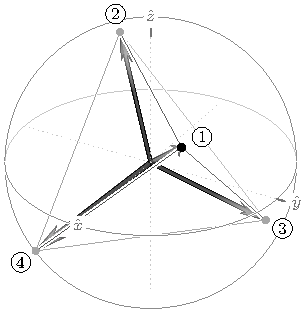
\includegraphics{figures/recipe_tet_sphere.pdf}}}%
  \hfil
  \COL{276pt}{\CTR{276pt}{\RecipeMasterTable}%
    \NIS{4pt}%
    \PBOX{276pt}{$V=4$;
      $\sum_k E_k=\Id$; $\Tr E_k=\tfrac12$; each rank one;
      $|\braket{\psi_j}{\psi_k}|^2=\tfrac13$ for $j\neq k$: the SIC condition,
      at the Welch bound.}}%
}%
\BANDRULE
%
% --- band B: steps 2, 3 and 4 ----------------------------------------------
% Head 2 names the dashed box and says it is off: everything printed in this
% band---the four probabilities, the bits, the outcome key---is the circuit
% run WITHOUT the U_g prefix, and the alpha^2 claim below is only true so.
% Head 3 gives the bit order, because a reader who takes the bits
% data-wire-first swaps vertices 2 and 3 on every shot; ancilla-first (top
% wire) is Table D.4's own convention and what assertion 9's rebuild returns.
\FULLHEAD{2}{Run this circuit, step~5's dashed box omitted; measure both
  wires.}%
  {Figure~\ref{fig:tet_povm_circuit} $\cdot$ Appendix~\ref{app:decker}}%
\NIS{2pt}%
\FULLHEAD{3}{Read the two bits, top wire first, as a vertex.}%
  {Table~\ref{tab:decker-labels}}%
\NIS{4pt}%
\hbox to \hsize{%
  \COL{306pt}{\hbox to 306pt{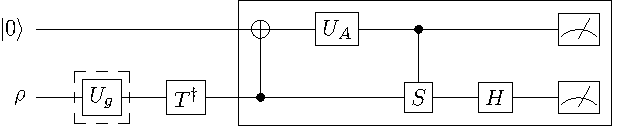
\includegraphics{figures/recipe_tet_circuit.pdf}\hss}}%
  \hfil
  \COL{136pt}{\PBOX{136pt}{\RecipeCircuitParams}}%
}%
\NIS{3pt}%
% The opening clause is the one sentence on the page that says what a
% reorientation IS (the strip's "reorientation exact?" column is unparseable
% without it); the generator checks it off the rebuilt circuit (check 9: the
% box without T-dagger measures our effects turned 45 degrees about z).
% The exactness sentence is the thesis's own (Sections 4.2.2 and 5.1) and each part
% of it is load-bearing: the italic on \textit{deterministic}, without which
% the two clauses read as a flat contradiction; the parenthetical "any
% dilation, this one included", which is what says the circuit printed just
% above is not exact; and "admits an exact implementation", which must not be
% reduced to a pronoun.  Four lines.  What paid for the opening clause is
% "each also the top-left entry of its own E_k" --- the master table's last
% head now reads <0|E_k|0>, which says the same thing beside the matrices.
\PBOX{\hsize}{$T^\dagger$ reorients the published circuit, the solid box, to
  our pose. On $\rho=\ketbra{0}{0}$ the data wire is untouched until the
  final $H$, so the four probabilities are $\alpha^2,\alpha^2,\beta^2,\beta^2$:
  the $\bra{0}E_k\ket{0}$ column above---but no \textit{deterministic}
  protocol over any gate set of this thesis---any dilation, this one
  included---implements any Platonic solid POVM exactly
  (Theorem~\ref{thm:main}); only the octahedral POVM admits an exact
  implementation, exhibited by the coin below, $\{\Id, \mathbf F, \mathbf F^\dagger\}$.}%
\NIS{4pt}%
\FULLHEAD{4}{Predict $p(k)=\Tr[E_k\rho]=\tfrac14(1+\hat n_k\cdot r)$; or
  invert, $r=3\sum_k p(k)\hat n_k$.}%
  {Section~\ref{sec:platonic-solid-povms} $\cdot$ Appendix~\ref{sec:shadows:setup}}%
\BANDRULE
%
% --- band C: steps 5 and 6 -------------------------------------------------
% Head 5 defines the rotation table's last column: the reading, g^{-1}.
\FULLHEAD{5}{Rotate it: prepend one atlas word; outcomes $1234$ then read as
  its row.}%
  {Table~\ref{tab:binary-tetrahedral-group-2t} $\cdot$ Section~\ref{subsec:rotated-povms}}%
\NIS{2pt}%
\FULLHEAD{6}{Twirl: draw that word uniformly.}%
  {Section~\ref{subsec:randomized-implementations} $\cdot$ Appendix~\ref{sec:shadows:channels}}%
\NIS{4pt}%
\hbox to \hsize{%
  \COL{156pt}{\RecipeRotationTable}%
  \hfil
  \COL{290pt}{\CTR{290pt}{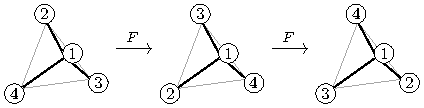
\includegraphics{figures/recipe_tet_frames.pdf}}%
    \NIS{3pt}%
    \PBOX{290pt}{$F$ turns the labelled solid $120^\circ$ about
      vertex~1's axis; twice is pair~3, a third brings it home---but
      $\mathbf F^3=-\Id$. Pairs 4, 5, 10 turn $180^\circ$.\par\vskip3pt
      Twelve rotations, twenty-four unitaries: each pair is one rotation and
      two atlas words $\pm U$---pair~2 is $\mathbf F$ and
      $\mathbf F^\dagger\mathbf F^\dagger=-\mathbf F$, both
      $1234\mapsto1342$.\par\vskip3pt
      Two permutations make one: $Z$ then $X$, or $X$ then $Z$, is pair~10's
      half-turn about $\hat y$---but $\mathbf{XZ}=-\mathbf{ZX}$; the order
      shows up only as the sign.\par\vskip3pt
      Prepending $U_g$ rotates the effects by $g^{-1}$: with $F$, outcomes
      $1,2,3,4$ read as vertices $1,3,4,2$. Drawn afresh each shot and
      relabelled, that is
      \hyperref[subsec:randomized-implementations]{\textit{twirled-native}},
      and measurement-side noise then averages to depolarizing.}}%
}%
\BANDRULE
%
% --- band D: the series strip ----------------------------------------------
\CTR{\hsize}{\RecipeSeriesStrip}%
}%
